% tog-sample.tex, dated 25th May 2012
% This is a sample file for ACM Transactions on Graphics
%
% Compilation using 'acmtog.cls' - version 1.2, Aptara Inc.
% (c) 2010 Association for Computing Machinery (ACM)
%
% Questions/Suggestions/Feedback should be addressed to => "acmtexsupport@aptaracorp.com".
% Users can also go through the FAQs available on the journal's submission webpage.
%
% Steps to compile: latex, bibtex, latex latex
%
% For tracking purposes => this is v1.2 - May 2012
\documentclass{acmtog}


% Package to generate and customize Algorithm as per ACM style
\usepackage[ruled]{algorithm2e}
\usepackage{amsfonts} % for mathbb
\renewcommand{\algorithmcfname}{ALGORITHM}
\newcommand{\indentitem}{\setlength\itemindent{25pt}}
\SetAlFnt{\small}
\SetAlCapFnt{\small}
\SetAlCapNameFnt{\small}
\SetAlCapHSkip{0pt}
\IncMargin{-\parindent}

\acmVolume{VV}
\acmNumber{N}
\acmYear{YYYY}
\acmMonth{Month}
\acmArticleNum{XXX}  
\acmdoi{10.1145/XXXXXXX.YYYYYYY}

\acmVolume{28}
\acmNumber{4}
\acmYear{2009}
\acmMonth{August}
\acmArticleNum{106}  
\acmdoi{10.1145/1559755.1559763}

\begin{document}

\markboth{Gainey, Seth Rylan}{Return To Normality: A Statistical Analysis of the Netflix Training Dataset}

\title{Return To Normality: A Statistical Analysis of the\\ Netflix Training Dataset} % title

\author{Gainey, Seth Rylan
\affil{Southern Methodist University;\\ Space {and} Naval Warfare Systems Center Charleston}
}

\category{G.3}{Probability and Statistics}{Distribution functions}[Normal Distribution]

%\terms{Data Mining}

\keywords{Kolmogorov-Smirnov, Non-Parametric, Long Tail, Netflix}

%\acmformat{Gainey, Seth Rylan. 2012. Return To Normality: A Statistical Analysis of the Netflix Training Dataset.}

\maketitle

\begin{bottomstuff}
This work is submitted in partial fulfillment of the requirements of EMIS7300, taught in Fall 2012 at Southern Methodist University under the guidance of Dr. Thomas Siems.

Author's addresses: S. Gainey, Systems Engineering Department,
Bobby Lyle School of Engineering, Southern Methodist University;
Enterprise Systems Engineering, Space and Naval Warfare Systems Center Charleston.
\end{bottomstuff}



\begin{abstract}
The movie ratings in the Netflix Prize training dataset represent the largest data release provided to the public from the internal records of a for-profit company; it contains the anonymized rating activities of 480,189 customers over 7 years (October 1998--December 2005). An analysis of this data for patterns following a normal probability distribution indicates that the majority of customer activies follow power law or mixture model distributions, but the average movie rating per customer and the average rating per movie conform to Gaussian curves. In addition, the mean of this customer rating curve increases for each year, implying systemic changes in Netflix customer base or customer behavior.
\end{abstract}

\section{Motivation \& Background}
\medskip
\begin{quote}
``[N]ature has established patterns originating in the return of events,\\
 . . . but only for the most part."\\

\hspace{5em}---\textit{Leibniz in response to Bernoulli, 1703}
\end{quote}
Choice of dataset for normality tests was based on 1) preference for "non-natural" data and 2) preference for large datasets ($>$1,000,000 data points). While normal probability distributions are typical throughout nature \cite{bernstein:against}, they are primarily associated with physical attributes and, in some cases, social structures. The chests sizes of Scottish soldiers (cf. Quetelet) will conform to random---rather than systemic---variation, but their incomes, personal library sizes and film predilections will tend towards non-normal distributions.
\\
\\
A large dataset was chosen to not only validate the Law of Large Numbers, but also to test the limits of data manipulation on the author's computing systems.
\\
\\
The Netflix dataset has been used for academic and competitive projects related to predication and data-mining methods, but never to analyze the distribution of data provided by processes suspect to human reliability. Answers to these questions can lead to insight on the probabilistic nature of rating systems and the vagaries of human opinion.

\section{Dataset Introduction}

In 2006, Netflix announced the \$1-million Netflix Prize, an open competition for improving their rating prediction algorithm. In an unprecedented act of data-sharing, the company released 100,480,507 movie ratings, created by 480,189 customers. This data---when converted to a normalized relational format (see steps in \S4)---amounts to 5GB of data. Shortly after release, researchers found by combining the anonymized Netflix data with public IMDB profiles, one could interpolate the real world identities of the Netflix customers and information related to their movie rentals \cite{DBLP:journals/corr/abs-cs-0610105} including information such as political affiliation and sexual orientation \cite{Wired-01}. The dataset has since been withdrawn due to legal liability, but is still available from third parties \cite{netflix-01}.

\medskip

\section{Questions \& Result Summary}

For each metric in table~\ref{table:one}, this paper presents a Kolmogorov-Smirnov test of its conformation to a normal distribution, along with a calculation of the mean, standard deviation; skew and kurtosis are provided for normal distributions, and the median is provided for non-normal distributions.

\begin{table}
\begin{center}
    \begin{tabular}{ | p{1.6cm} | p{2.8cm} | p{2.8cm} |}
    \hline
    \textsc{Metric} & \textsc{Explanation} & \textsc{Result} \\ \hline
    Average Rating by Customer &  Probability of a user with an average given rating of r. \textbf{What is an average customer?} & Normal, with $\mu=$ 3.674 and $\sigma=$ 0.473. \\ \hline
    Average Rating by Movie & Probability of a movie with an average given rating of r. \textbf{What is the threshold for a ``good" movie?}  & Near-normal (bimodal), with a single Gaussian approximate at $\mu=$ 3.228 and $\sigma=$ 0.526. \\ \hline
   Number of Ratings per Customer & Probability of a customer rating r number of movies. \textbf{What is a ``prolific" customer?} & Non-normal with long tail; $\mu=$ 210 and median $=$ 96. \\ \hline
    Number of Ratings per Movie &  Probability of a movie having r number ratings. \textbf{What is ``a lot" of ratings?} & Non-normal with long tail; $\mu=$ 5655 and median $=$ 561  \\
    \hline
    \end{tabular}
\textsc{Research Objectives}
\end{center}
\caption{}
\label{table:one}
\end{table}

\medskip

\section{Methodology}

\subsection{Data Preprocessing}

The steps for preparing the environment and importing the Netflix dataset into a relational format require 8--12 hours, depending on the speed of the computer and network connections. The compressed dataset \cite{netflix-01} accounts for {\raise.17ex\hbox{$\scriptstyle\mathtt{\sim}$}}2GB. After extraction, there are four separate data types, but only two are needed for the purposes of the research objectives: movie titles (n = 17770, stored in a single text file with title and release year) and the training set (one file per movie, listing customer ID's, ratings and date of rating). Dates are in format YYYY-MM-DD, ratings range from integer values 1 to 5, and customer ID's range from from 1 to 2649429, with gaps (480,189 total customers).


\begin{figure}
\centerline{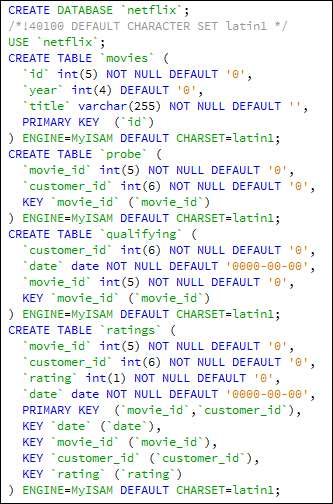
\includegraphics[scale=.6]{01schema.png}}
\caption{SQL DDL for schema creation}
\label{fig:one}
\end{figure}

\subsubsection{Software Versions Used} Available without restriction on most platforms.
\begin{itemize}
	{\indentitem\item Python 2.7.3 (32-bit)}
	{\indentitem\item Ruby 1.93 (32-bit)}
	{\indentitem\item MySQL 5.5 (32-bit)}
	{\indentitem\item NumPy 1.6.2 (32-bit)}
	{\indentitem\item matplotlib 1.2.0 (32-bit)}
	{\indentitem\item SciPy 0.11.0 (32-bit)}
\end{itemize}
\subsubsection{MySQL Configuration} Default values shown where exists.
\begin{itemize}
	{\indentitem\item query\_cache\_size = 0 $->$ 100M}
	{\indentitem\item query\_cache\_limit = 3M}
	{\indentitem\item myisam\_sort\_buffer\_size = 69M -$>$ 200M}
	{\indentitem\item bulk\_insert\_buffer\_size = 100M}
	{\indentitem\item join\_buffer\_size = 100M}
	{\indentitem\item key\_buffer\_size = 55M -$>$ 600M}
	{\indentitem\item read\_buffer\_size = 64K -$>$ 200M}
	{\indentitem\item sort\_buffer\_size = 256K -$>$ 500M}
	{\indentitem\item disable InnoDB/transaction support by using myisam storage engine.}
\end{itemize}

\subsubsection{Schema Defintion}
The schema used for storing the normalized dataset is based on versions used by other researchers \cite{igvita-01}; the specific code used for this example can be seen in Figure~\ref{fig:one}.

\begin{figure}
\centerline{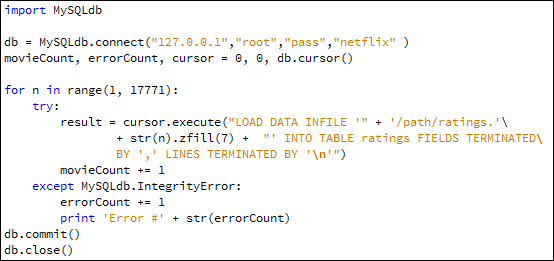
\includegraphics[scale=.6]{04load.png}}
\caption{Python code for final database load}
\label{fig:two}
\end{figure}

\subsubsection{Import Optimization}
The 17770 ratings files must be flattened and converted into raw SQL format and then imported using a raw DATA LOAD. The final import can be reduced from over 28 hours to {\raise.17ex\hbox{$\scriptstyle\mathtt{\sim}$}}3 hours using this method (see code in Figure~\ref{fig:two}).


\subsection{Aggregate Data Queries}

Despite the work done in the previous steps to optimize the dataset for querying, each SQL aggregate functions used in this section can take 45--150 minutes to complete.
\begin{enumerate}
	\item Average Rating by Customer \\ \\
		$select$ $avg$(rating) $from$ ratings $group\ by$ customer\_id;
		\\

	\item Average Rating by Movie \\ \\
		$select$ $avg$(rating), title $from$ ratings $inner\ join$ movies $on$ movies.id$=$ratings.movie\_id $group\ by$ movie\_id;
		\\

	\item Number of Ratings per Customer \\ \\
		$select$ $count$(*), customer\_id $from$ ratings $group\ by$ customer\_id;
		\\

	\item Number of Ratings per Movie \\ \\
		$select$ $count$(*), title $from$ ratings $inner\ join$ movies $on$ movies.id$=$ ratings.movie\_id $group\ by$ movie\_id;
		\\

\end{enumerate}

\subsection{Processing, Analysis, Statistics \& Graphics}
Normalization of the data array for the Kolmogorov-Smirnov (K-S) test is performed by mapping the function
\begin{equation}
x_{i,norm}=(x_i-\mu)/\sigma
\end{equation}
\\to the set of values used to create the probability density function.
\\
\\
The one-sample Kolmogorov-Smirnov test is used in each distribution to test the goodness-of-fit of the normalized data to a Gaussian curve of $\mu=0, \sigma=1$, using the equation:

% Numbered Equation
\begin{equation}
\label{eqn:k-s}
D = max_{i\leq i\leq n}\left ( F(Y_i) - \frac{i-1}{N},\frac{i}{N}-F(Y_i)) \right )
\end{equation}\\\\
where $F()=\phi()$, the standard normal distribution.
\\
%A^2 = -n - \sum_{k=1}^{n} (\frac{2k-1}{n})[ln(F(Y_k))+ln(1-F(Y_{n+1-k}))]
%W = \frac{(\sum_{i=1}^{n}a_ix_i)^{2}}{\sum_{i=1}^{n}(x_i-\mu)^{2}}
\\
The null hypothesis $H_0$ is that the distribution came from a normally distributed population; $H_a$ is that the data does not follow the normal distribution. All tests use significance level $\alpha=$ .05
\cite{korn:handbook}.
\\
\\
Functions from the NumPy, SciPy and matplotlib libraries produce the calculated values and graphics in later sections. A simplified version is shown in Figure~\ref{fig:code}.

\begin{figure}
\centerline{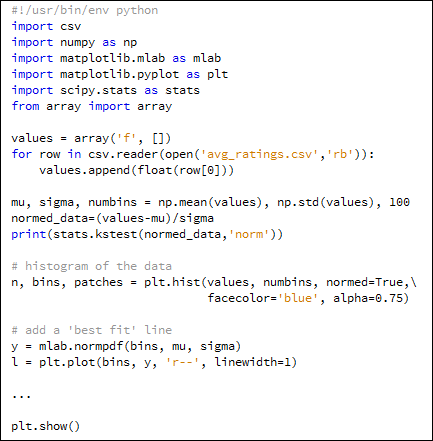
\includegraphics[scale=.6]{code_sample.png}}
\caption{Code Sample for Data Manipulation}
\label{fig:code}
\end{figure}

\medskip

\section{Results}

\subsubsection{Note on histogram normalization}Where not otherwise stated, the number of histogram bins are calculated based on the code in Algorithm~\ref{alg:one}; when the number of bins is greater than the domain, this approach can produce histogram bars with a height greater than 1.0, however the reader can verify through trapezoidal integration that the area of the PDF curve totals to 1.0. Each PDF of a normal distribution has an overlayed plot of an ideal Gaussian curve (red dashed line) from the calculated $\mu$ and $\sigma$ of the dataset.

\begin{algorithm}[t]
\SetAlgoNoLine
\KwIn{Non-normalized values}
\KwOut{Weight value such that integrated area of bins equals normalized area}
normalizedarea, minval, maxval $=$ 1, min(values), max(values; \newline
binweight = normalizedarea * numbins / (maxval-minval) / values.size; \newline
\caption{Histogram Normalization Algorithm}
\label{alg:one}
\end{algorithm}

\subsection{Average Rating by Customer}

\begin{figure}
\centerline{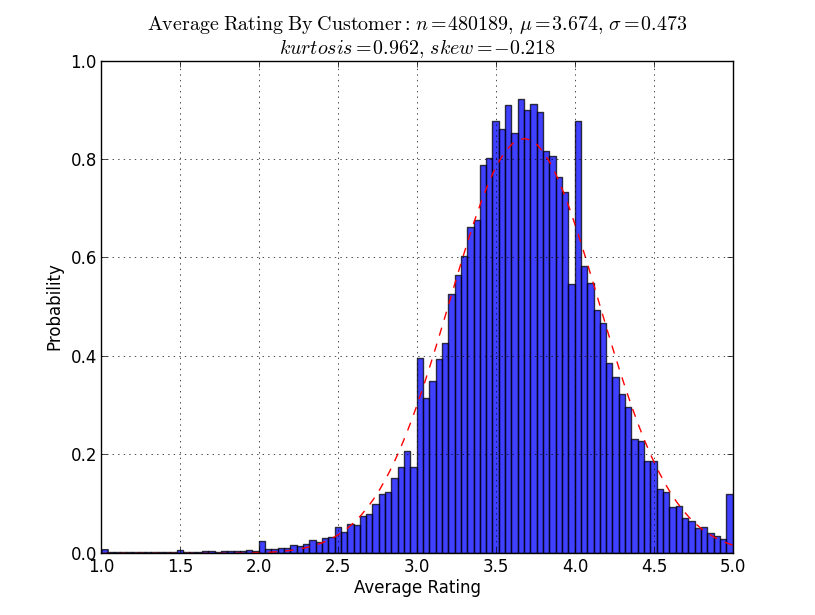
\includegraphics[scale=.5]{average_rating_by_customer.png}}
\caption{Probability Density Function (PDF) of the Average Rating Score Given by Customer}
\label{fig:three}
\end{figure}

The average of all given ratings by each customer (Figure~\ref{fig:three}) provides the closest approximation to a normal probability distribution found in the Netflix dataset. Peaks exist at each integer value ([1,2,3,4,5] $\epsilon \mathbb{Z}$), preceeded by dips at values immediately below; the result of customer habits to assign uniform ratings. The distribution is slightly leptokurtic (i.e., more ``peaky" than true normal), indicating a central tendency.
\\
\\
From the K-S test, D $=$ 0.0200  ($<\alpha$ = .05); $H_0$, that the data is normally distributed, is not rejected.


\subsection{Average Rating by Movie}

\begin{figure}
\centerline{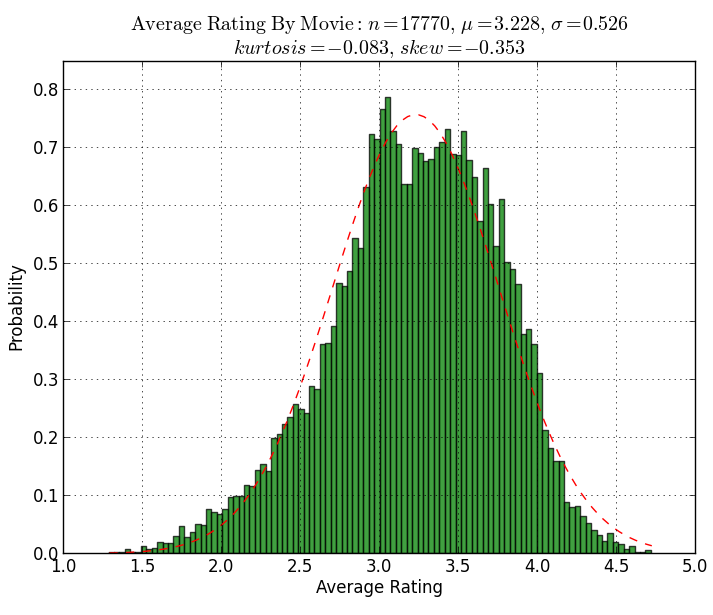
\includegraphics[scale=.45]{average_rating_by_movie.png}}
\caption{Probability Density Function (PDF) of the Average Rating Score by Movie}
\label{fig:four}
\end{figure}

The average of all given ratings to each movie (Figure~\ref{fig:four}) comes close to a normal distribution, with slight negative skew (i.e., right ``leaning"). There is lower than normal probability for a movie to have a rating between 3.2 and 3.4, indicating a bimodal distribution. The author recommends the application of Gaussian Mixture models for future work, but there are two possible explanations presented.

\begin{table}
\begin{center}
    \begin{tabular}{ | l | l | l |  l | l |  l  |}
    \hline
    \textsc{Year} & \textsc{Ratings ($n$)} & $\mu$ & $\sigma$ & \textsc{Skew} &  \textsc{Kurtosis} \\ \hline
    1999 & 2,178         & 3.337 & 1.161 & -0.305 & -0.646 \\ \hline
    2000 & 924,443     & 3.365 & 1.124 & -0.316 & -0.570 \\ \hline
    2001 & 1,769,031  & 3.391 & 1.104 & -0.336 & -0.521 \\ \hline
    2002 & 4,342,871  & 3.382 & 1.103 & -0.351 & -0.502 \\ \hline
    2003 & 9,985,337  & 3.406 & 1.100 & -0.377 & -0.478 \\ \hline
    2004 & 30,206,574& 3.595 & 1.079 & -0.501 & -0.313 \\ \hline
    2005 & 53,250,073& 3.676 & 1.074 & -0.554 & -0.256  \\ \hline
    \end{tabular}
\\
\textsc{Time-series Metrics}
\end{center}
\caption{}
\label{table:two}
\end{table}

\begin{enumerate}
	\item A cursory analysis suggests that customers tend to rate movies as exclusively ``good" or ``bad"; there are many movies rated as 4's and 5's, and many movies rated as 1's, 2's, and 3's; but relatively few movies rated as ``ok" at 3's and 4's. In other words, customers tend to rate movies for which they hold strong opinions.
	\item When analyzing the time-series data (table~\ref{table:two}), there is a distinct yearly trend towards higher ratings with less variation. Systemic changes in customer-base or behavior likely cause this pattern, and the collapse of these time-domain stratifications, combined with a increase in number of customers or rating frequency, may produce the bimodal distribution.
\end{enumerate}
Despite this deviation, from the K-S test, D $=$ 0.0295 ($<\alpha$ = .05); $H_0$, that the data is normally distributed, is not rejected.



\subsection{Number of Ratings per Customer}

\begin{figure}
\centerline{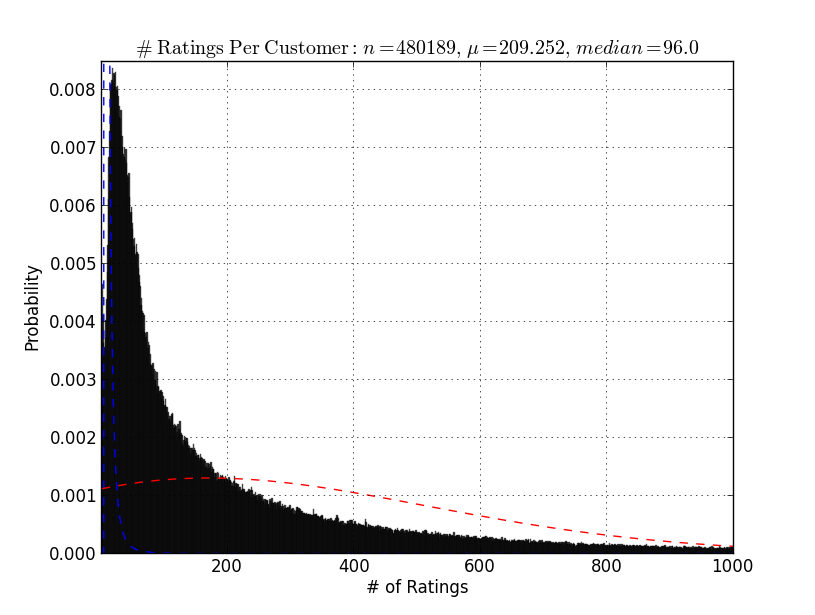
\includegraphics[scale=.45]{num_ratings_per_customer.png}}
\caption{Probability Density Function (PDF) of the Number of Ratings per Customer. Note: this figure uses a unity number of bins (\# of bins equal to x-axis domain and merged); therefore the y-axis probabilities are normalized to 1 for each integer value.}
\label{fig:five}
\end{figure}

The number of ratings per customer (Figure~\ref{fig:five}) has a arithmetic mean of 210 and a median of 96. The Long Tail of the graph (values over 1000 are not shown, but the maximum number of ratings is 17653) indicates a more exotic distribution. Lognormal and rayleigh (Weibull special case, with $\delta = 2$) PDFs---shown in blue and red respectively---were fitted using the SciPy library but fail to approximate the distribution. The fitting method used by SciPy weighs long tail values and peak values equally, and therefore the curve fits appear non-optimal in Figure~\ref{fig:five}.
\\
\\
From the K-S test, D $=$ 0.245 ($>\alpha$ = .05); $H_0$, that the data is normally distributed, is rejected.

\subsection{Number of Ratings per Movie}

\begin{figure}
\centerline{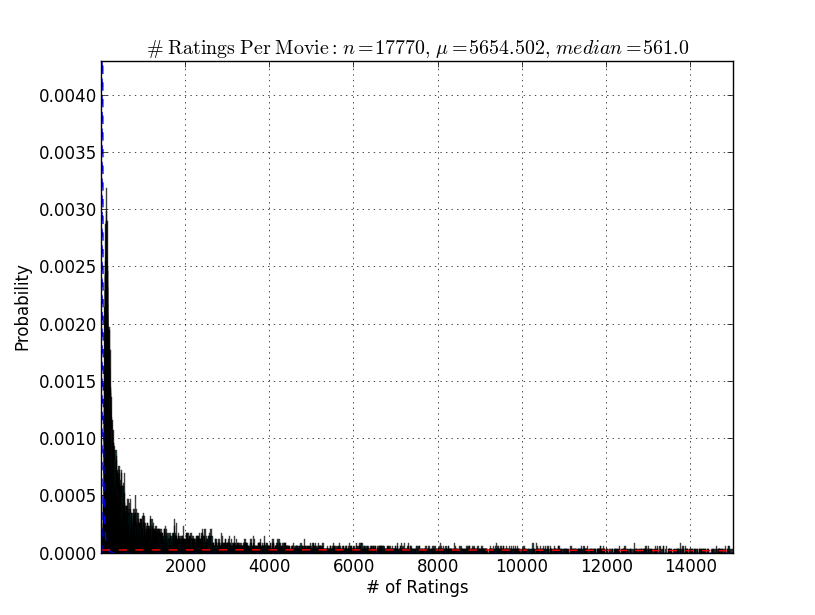
\includegraphics[scale=.45]{num_ratings_per_movie.png}}
\caption{Probability Density Function (PDF) of the Number of Ratings per Movie. Note: this figure uses a unity number of bins (\# of bins equal to x-axis domain); therefore the y-axis probabilities are normalized to 1 for each integer value.}
\label{fig:six}
\end{figure}

The number of ratings each movie receives (Figure~\ref{fig:six}) does not follow a normal distribution; the arithmetic mean is 5654 and the median is 561. The lognormal and rayleigh PDF curves of best fit are shown in blue and red. Values above 15,000 are not displayed, but the Long Tail extends into 100,000's: \textit{The Patriot} (200,832), \textit{Independence Day} (216,596) and \textit{Miss Congeniality} (232,944) are the most rated movies from the dataset.
\\
\\
From the K-S test, D $=$ 0.369 ($>\alpha$ = .05); $H_0$, that the data is normally distributed, is rejected.
\medskip
\section{Conclusion \& Reflection}

\subsection{Overview}
Analysis of the Netflix dataset has shown that most derived attributes related to movie ratings will follow power law distributions, and discovering normal distributions in the data has been a challenging problem to solve, especially given the scale of the data. The investigation presented in this paper omits several failed attempts at modelling the dataset. 
\\
\\
In general, distributions of data with no fixed minimum or maximum values will produce non-normal distributions. This explains why physical limits produce normal distributions of body size/weight, but not income, and why only the distributions of ratings (limited in range from 1.0 to 5.0) followed a normal curve. There exist inherent limits to the height of the world's tallest person, but not to the wealth of the world's richest; nor, apparently, to the number of films he or she is capable of rating.

\subsection{Comments on Distribution Mixture Models}
For the distributions which did not conform to normal, lognormal or rayleigh distributions, it is suspected that there is a mixture of power law and normal-like distributions to account for the initial peak and very long tail of the data.

\subsection{Comments on Outliers}
Some of the outliers in the plot of highly rated movies (not shown) include the extended editions of \textit{Lord of the Rings} trilogy, at respective average ratings of 4.7026, 4.7166, and 4.7233. While the standard editions of these films did nearly as well, a customer is unlikely to watch extended version sequels without first enjoying the standard edition prequels, and is therefore more likely than to enjoy the movie. Notably, the \textit{Star Wars} releases do not show the same pattern, for reasons left as an exercise for the reader.

\subsection{Reflection on Technical Challenges}
Data analysis proved very challenging; the more robust Anderson-Darling and Shapiro-Wilk normality tests were discarded due to difficulty in implementation. Methods for visualizing time-series distributions also failed to produce adequate results.
\\
\\
In many cases, it was found that a data structure useful for quickly producing graphs of 17,770 values would dissapoint at 100,000$+$, because the time to completion grew with an exponential relationship to $n$. The time to re-write and re-run the algorithm with an optimized data structure required far less time than the original program would have needed to complete. The lessons of Knuth come to mind:

\begin{quote}
``We should forget about small efficiencies, say about 97\% of the time: \textbf{premature optimization is the root of all evil}. Yet we should not pass up our opportunities in that critical 3\%. A good programmer will not be lulled into complacency by such reasoning, he will be wise to look carefully at the critical code; but only after that code has been identified."\\

\hspace{5em}---\textit{Donald Knuth}, emphasis added \cite{knuth-01}
\end{quote}

\medskip


% Bibliography
\bibliographystyle{acmsmall}
\bibliography{acmsmall-sam}


\medskip




\bibliographystyle{acmtog}
\bibliography{acmsmall-sam}


\received{September 2008}{March 2009}

\end{document}
